\documentclass[10pt,a4paper]{article}
\usepackage{needspace}
\usepackage[nobottomtitles]{titlesec}
\usepackage{multicol}
\usepackage{xcolor}
\usepackage{fp}
\usepackage{xfp}
\usepackage{enumitem}
\usepackage[version=4]{mhchem}
\usepackage{WriteOnGrid}
\usepackage{frcursive}
\usepackage{csvsimple}%
\usepackage[francais,bloc]{automultiplechoice}

\FPseed=10

\baremeDefautS{e=0,v=0,b=1,m=-.1}
\baremeDefautM{e=0,v=0,b=.5,m=-.1}

\graphicspath{ {./images/} }

\newenvironment{reponsesd}{
    \begin{multicols}{2}
    \begin{reponses} }{
    \end{reponses}
    \end{multicols}
}

\setlength{\columnseprule}{1pt}
\def\columnseprulecolor{\color{lightgray}}%

\let\oexplain\explain
\renewcommand{\explain}[1]{\oexplain{\textcolor{red}{#1}}}

\titleformat{\section}
  {\centering\hrule\vspace{2mm}}
  {\thesection}
  {1em}
  {}
  [\vspace{1mm}\hrule]

\titleformat{\subsection}
  {\em}
  {\thesubsection}
  {1em}
  {}

\newcommand{\sujet}{
\exemplaire{1}{%

\AMCsetFoot{\niveau{} \classe{} -- \prenom{}~\nom{} -- \thepage}

%%% debut de l'en-tête des copies :
\begin{center}
\vfill
\noindent{\large \bf Classe de \niveau{}°\classe{}}

\vspace*{3mm}

{\Large\bf Évaluation de compétences (non notée) STL - Physique-Chime 15/10/2025}

\vfill
\namefield{\noindent{}\fbox{\vspace*{3mm}
         \Huge\bf\prenom{}~\nom{}\normalsize{}%
         \vspace*{3mm}
      }}
\end{center}
\vfill

\begin{center}
\textbf{Durée : 30 minutes.}
\vspace*{5mm}

  Aucun document n'est autorisé.
  L'usage de la calculatrice est interdit.

  Les questions faisant apparaitre le symbole \multiSymbole{} peuvent
  présenter une ou plusieurs bonnes réponses. Les autres ont
  une unique bonne réponse.

  {\color{white} Des points négatifs seront affectés aux mauvaises réponses.}
  \vspace*{5mm}

  \textbf{IMPORTANT: Utilisez un crayon de papier bien noir pour cocher les cases, et une gomme pour effacer délicatement en cas d'erreur. Ne raturez pas les cases. Si vous effacez le pourtour de la case, ne le redessinez pas!}

  \vspace*{5mm}

  Ne pas faire comme ceci (pas centré, trop pâle, raturé):\\
  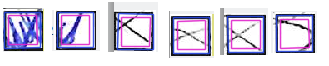
\includegraphics[width=4cm]{checkbox_bad.png}

  Mais comme cela (bien centré, bien foncé):\\
  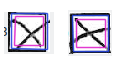
\includegraphics[width=2cm]{checkbox_good.png}

  Si vous faites une erreur et que vous ne pouvez effacer, raturez la case bien ostensiblement.

\end{center}
\vspace{1ex}
\vfill
\pagebreak
%%% fin de l'en-tête

\restituegroupe{groupes}


\AMCassociation{\id}

	  } % End \exemplaire{1}{%
} % End \newcommand{\sujet}{


%%%%§§§§§§§§§§§§§§§§§§§§§§§§§§§§§§§§§
\newcommand{\allq}{}
\newcommand{\nball}[1]{#1}

\begin{document}
%%%Options
\AMCrandomseed{10}

\def\AMCformQuestion#1{{\sc Question #1 :}}

\setdefaultgroupmode{withoutreplacement}
%%% Fin Options

%%% elements

\element{meta}{
  \begin{question}{meta1}\QuestionIndicative
    Pensez-vous poursuivre vos études dans un domaine lié à la physique, la chimie ou la biologie~?
    \begin{reponses}[o]
      \bonne{Oui}
      \bonne{Peut-être}
      \bonne{Ne sait pas}
      \bonne{Probablement pas}
      \bonne{Non}
    \end{reponses}
    \explain{C'est votre choix.}
  \end{question}

  \begin{question}{meta2}\QuestionIndicative
    Si oui, plutôt dans quel domaine (et sinon, quoi)~?
    \begin{reponses}[o]
      \bonne{Physique}
      \bonne{Chimie}
      \bonne{Biologie}
      \bonne{Autre, précisez: }
    \end{reponses}
    \explain{C'est votre choix.}
  \end{question}

  \begin{question}{meta3}\QuestionIndicative
    Que vous souhaitiez en faire votre métier ou non, aimez-vous la physique, la chimie ou la biologie~?
    \begin{reponses}[o]
      \bonne{Oui}
      \bonne{Un peu}
      \bonne{Ne sait pas}
      \bonne{Pas trop}
      \bonne{Non}
    \end{reponses}
    \explain{C'est votre choix.}
  \end{question}

  \begin{questionmult}{meta4}\QuestionIndicative
    Que préférez-vous (plusieurs choix possibles)~?
    \begin{reponses}[o]
      \bonne{Physique}
      \bonne{Chimie}
      \bonne{Biologie}
      \bonne{Mathématiques}
      \bonne{Autre, précisez: }
    \end{reponses}
    \explain{C'est votre choix.}
  \end{questionmult}

} % End \element{meta}{

\element{strspc}{
  \begin{questionmult}{strspc1}
    Une molécule est dite chirale si~:
    \begin{reponses}
      \mauvaise{ses atomes sont alignés}
      \mauvaise{elle est superposable à son image dans un miroir}
      \mauvaise{ses énantiomères sont diastéréoisométriques}
      \bonne{elle n'est pas superposable à son image dans un miroir}
    \end{reponses}
    \explain{un composé est dit chiral s'il n'est pas superposable à son 
    image dans un miroir plan.}
  \end{questionmult}
}

\element{strspc}{
  \begin{questionmult}{strspc2}
    La conformation d'une molécule se défini par~:
    \begin{reponses}
      \mauvaise{ses caractéristiques isomérique}
      \mauvaise{son respect des spécifications de son espèce chimique}
      \mauvaise{la qualité de son image dans un miroir plan}
      \bonne{les arangement des atomes tournant autour de liaisons simples}
    \end{reponses}
    \explain{La conformation d'une molécule correspond à l'orientation des atomes autour
    de liaisons simples. Celle-ci pouvant la plupart du temps tourner librement, 
    le même composé chimique peut passer de une à l'autre facilement.}
  \end{questionmult}
  }

\element{strspc}{
  \begin{questionmult}{strspc3}
    La configuration d'une molécule est~:
    \begin{reponses}
      \mauvaise{la version de système d'exploitation installé par défaut}
      \mauvaise{les arangement des atomes tournant autour de liaisons simples}
      \mauvaise{son image dans un miroir plan}
      \bonne{la disposition de ses atomes dans l'espace indépendamment des rotations
      autour des liaisons simples}
    \end{reponses}
    \explain{La configuration d'une molécule correspond à l'orientation des atomes dans l'espace,
    indépendamment des rotations autour des liaisons simples. Pour changer de configuration,
    il faut casser des liaisons pour en reformer d'autres.}
  \end{questionmult}
}

\element{strspc}{
  \begin {questionmult}{strspc4}
    Deux molécules sont des stéréo-isomères chimiques, si~:
    \begin{reponses}
      \mauvaise{elles ont une formule brute différente mais les mêmes propriétés chimiques}
      \mauvaise{elles ont la même conformation}
      \mauvaise{elles ont la meme configuration mais une formule semi-développée differente}
      \bonne{elles ont même formule semi-développée mais une configuration différente}
    \end{reponses}
    \explain{Les stéroisomères chimiques sont des molécules ayant la même formule
    semi-développée mais une conformation ou une configuration différente.}
  \end {questionmult}
}

\element{strspc}{
  \begin {questionmult}{strspc5}
    Deux molécules sont des énantiomères chimiques, si~:
    \begin{reponses}
      \mauvaise{elles ont même formule semi-développée mais ne sont pas images de l'une de l'autre dans un miroir plan}
      \mauvaise{elles ont la même mère}
      \mauvaise{la rotation de leur image dans un miroir dessine une ligne de symétrie}
      \bonne{elles sont images de l'une de l'autre dans un miroir plan}
    \end{reponses}
    \explain{Les enantiomères chimiques sont des molécules qui sont images de l'une de
    l'autre dans un miroir plan.}
  \end {questionmult}
}

\element{strspc}{
  \begin {questionmult}{strspc6}
    Deux molécules sont des diastéréoisométriques chimiques, si~:
    \begin{reponses}
      \mauvaise{elles ont une formule brute differente mais sont images de l'une de l'autre dans un miroir plan}
      \mauvaise{elles sont très très malades}
      \mauvaise{elles sont images de l'une de l'autre dans un miroir plan}
      \bonne{elles ont même formule semi-développée mais ne sont pas images de l'une de l'autre dans un miroir plan}
    \end{reponses}
    \explain{Les diastéréoisométriques .}
  \end {questionmult}
}

\element{nec}{
  \begin{questionmult}{nec1}
    À quoi servent les règles de Cahn, Ingold et Prelog en nomenclature chimique ?
    \begin{reponses}
      \mauvaise{Déterminer la conformation d'une molécule}
      \mauvaise{Établir les propriétés physiques d'un composé}
      \mauvaise{Déterminer si une molécule est chirale}
      \bonne{Donner la priorité aux substituents pour nommer les composés}
    \end{reponses}
    \explain{Les règles de Cahn-Ingold-Prelog permettent d'attribuer un ordre de priorité aux substituents afin de nommer correctement les composés chimiques.}
  \end{questionmult}
}

\element{nec}{
  \begin{questionmult}{nec2}
    Selon les règles de Cahn-Ingold-Prelog, comment détermine-t-on la priorité des substituents ?
    \begin{reponses}
      \mauvaise{En fonction du nombre de lettres dans le nom du substituant}
      \mauvaise{En fonction de la taille du substituant}
      \mauvaise{En fonction de la charge électrique du substituant}
      \bonne{En fonction du numéro atomique du premier atome du substituant}
    \end{reponses}
    \explain{La priorité est déterminée par le numéro atomique du premier atome du substituant. Si nécessaire, on examine les atomes suivants dans le substituant.}
  \end{questionmult}
}

\element{nec}{
  \begin{questionmult}{nec3}
    Qu'est-ce que la configuration R/S d'un centre chiral ?
    \begin{reponses}
      \mauvaise{Une classification des molécules en fonction de leur poids moléculaire}
      \mauvaise{Un système de désignation des isomères Z/E}
      \mauvaise{Une échelle de mesure de la polarité d'une molécule}
      \bonne{Un moyen de décrire l'arrangement spatial des substituents autour d'un atome}
    \end{reponses}
    \explain{La configuration R/S décrit l'arrangement tridimensionnel des quatre substituants différents autour d'un atome de carbone asymétrique.}
  \end{questionmult}
}

\element{nec}{
  \begin{questionmult}{nec4}
    Qu'est-ce que les désignations Z et E pour une double liaison ?
    \begin{reponses}
      \mauvaise{Elles indiquent si la molécule est droite ou gauche}
      \mauvaise{Elles classifient les molécules en fonction de leur solubilité}
      \mauvaise{Elles indiquent si la molécule est liquide ou gazeuse}
      \bonne{Elles décrivent la répartition des substituents de haute priorité autour d'une double liaison}
    \end{reponses}
    \explain{Z (zusammen) signifie que les substituents de plus haute priorité sont du même côté, tandis que E (entgegen) signifie qu'ils sont des côtés opposés.}
  \end{questionmult}
}

\element{acide}{
  \begin{questionmult}{acide1}
    Qu'est-ce qu'une constante d'équilibre acido-basique ?
    \begin{reponses}
      \mauvaise{Un paramètre qui mesure la vitesse d'un réaction chimique.}
      \mauvaise{Une valeur qui indique la température à laquelle une substance se décompose.}
      \mauvaise{C'est une unité de mesure pour les échelles de pH.}
      \bonne{Une constante qui décrit l'équilibre entre une espèce acide et 
      sa base conjuguée en solution aqueuse.}
    \end{reponses}
    \explain{La constante d'équilibre acido-basique est utilisée pour 
    quantifier la force relative d'un acide ou d'une base.}
  \end{questionmult}
}

\element{acide}{
  \begin{questionmult}{acide2}
    Qu'est-ce que le pKa, et à quoi sert-il ?
    \begin{reponses}
      \mauvaise{C'est un indicateur de la basicité d'une substance.}
      \mauvaise{C'est une mesure de la solubilité d'un composé dans l'eau.}
      \mauvaise{C'est l'abréviation pour 'pourquoi Kévin aime les acides'.}
      \bonne{C'est le logarithme négatif de la constante de dissociation acide, 
      servant à indiquer la force de l'acide.}
    \end{reponses}
    \explain{Un pKa élevé correspond à un faible acide, tandis qu'un pKa bas 
    indique un acide fort.}
  \end{questionmult}
}

\element{acide}{
  \begin{questionmult}{acide3}
    Comment le coefficient de dissociation est-il lié à la force d'un acide ?
    \begin{reponses}
      \mauvaise{Il n'y a pas de relation directe entre les deux.}
      \mauvaise{Un grand coefficient de dissociation indique un acide faible.}
      \mauvaise{Il est utilisé pour mesurer la quantité d'électricité dans une solution.}
      \bonne{Un grand coefficient de dissociation signifie que l'acide
      se dissocie plus facilement, ce qui en fait un acide fort.}
    \end{reponses}
    \explain{Le coefficient de dissociation reflète la proportion dans
    laquelle l'acide se sépare en ions en solution. Plus il est élevé, plus l'acide est fort.}
  \end{questionmult}
}

\element{acide}{
  \begin{questionmult}{acide4}
    Si un acide a un pKa de 5, qu'en déduisons-nous ?
    \begin{reponses}
      \mauvaise{Il s'agit d'un acide fort.}
      \mauvaise{Il est incapable de réagir avec une base.}
      \mauvaise{C'est un acide qui ne réagit qu'avec des bases naturelles.}
      \bonne{C'est un acide modérément faible}
    \end{reponses}
    \explain{Un pKa moyen comme 5 indique que l'acide n'est que très partiellement dissocié,
    ce qui est typique des acides faibles.}
  \end{questionmult}
}

\element{acide}{
  \begin{questionmult}{acide5}
    Quelle relation existe-t-il entre le pKa et la force d'un acide ?
    \begin{reponses}
      \mauvaise{Plus le pKa est élevé, plus l'acide est fort.}
      \mauvaise{Il n'y a pas de relation directe.}
      \mauvaise{Plus le pKa est élevé, plus l'acide est faible.}
      \bonne{Plus le pKa est bas, plus l'acide est fort.}
    \end{reponses}
    \explain{Un pKa bas signifie que l'acide se dissocie plus 
    facilement, ce qui en fait un acide fort.}
  \end{questionmult}
}

\element{acide}{
  \begin{questionmult}{acide6}
    Pourquoi les acides faibles ont-ils un coefficient de dissociation inférieur à 1 ?
    \begin{reponses}
      \mauvaise{Parce qu'ils ne sont pas capables de se dissocier.}
      \mauvaise{Parce que leur pKa est trop élevé.}
      \mauvaise{Parce qu'ils sont timides et n'osent pas se dissocier complètement.}
      \bonne{Parce qu'ils ne se dissocient pas complètement en solution aqueuse}
    \end{reponses}
    \explain{Les acides faibles partiellement se dissociie, donc leur coefficient
     de dissociation reste inférieur à 1.}
  \end{questionmult}
}


\element{tpco}{
  \begin{questionmult}{tpco1}
    Quelle est la principale fonction d'une solution tampon ?
    \begin{reponses}
      \mauvaise{Neutraliser complètement les acides et les bases forts.}
      \mauvaise{Agir comme catalyseur dans les réactions chimiques.}
      \mauvaise{Augmenter la conductivité électrique de l'eau.}
      \bonne{Résister aux changements de pH lorsqu'on ajoute de petites quantités
      d'acide ou de base.}
    \end{reponses}
    \explain{Les solutions tampon résistent aux variations du pH 
    en neutralisant les ions ajoutés grâce à leurs composants acido-basiques.}
  \end{questionmult}
}

\element{tpco}{
  \begin{questionmult}{tpco2}
    Comment les solutions tampon sont-elles généralement préparées ?
    \begin{reponses}
      \mauvaise{En mélangeant un acide fort avec une base forte.}
      \mauvaise{En ayant un certificat dûment tamponné.}
      \mauvaise{En dissolvant un solide dans l'eau pour créer une solution saturée.}
      \mauvaise{En chauffant un mélange d'acide et de base jusqu'à ébullition.}
      \bonne{En mélangeant un acide faible avec sa base conjuguée ou une base 
      faible avec son acide conjugué.}
    \end{reponses}
    \explain{Les solutions tampon sont préparées en combinant un 
    acide faible et sa base conjuguée.}
  \end{questionmult}
}

\element{tpco}{
  \begin{questionmult}{tpco3}
    Quel est le rôle du système de tampon bicarbonaté dans le sang ?
    \begin{reponses}
      \mauvaise{Réguler la température corporelle.}
      \mauvaise{Réguler la pression du sang.}
      \mauvaise{Transporter l'oxygène dans tout le corps.}
      \mauvaise{Digérer les aliments dans le sang.}
      \bonne{Maintenir le pH sanguin en neutralisant les ions 
      hydrogène en excès grâce à l'ion bicarbonate.}
    \end{reponses}
    \explain{Le système bicarbonaté aide à maintenir un pH stable
    dans le sang en neutralisant les excès d'acide ou de base.}
  \end{questionmult}
}

\element{tpco}{
  \begin{questionmult}{tpco4}
    Que se passe-t-il lorsque le CO2 se dissout dans l'eau ?
    \begin{reponses}
      \mauvaise{Il forme un acide fort qui se dissocie complètement.}
      \mauvaise{Il ne réagit pas et reste sous forme de molécules de \ce{CO2}.}
      \mauvaise{Il ne retrouve plus sa maison.}
      \mauvaise{Il réagit avec l'eau pour produire de l'oxygène.}
      \bonne{Il se dissout partiellement pour former de l'acide carbonique,
       qui se dissocie ensuite en ions \ce{H+} et bicarbonate (\ce{HCO3-}).}
    \end{reponses}
    \explain{Le \ce{CO2} se dissous réagit avec l'eau pour former une petite 
    quantité d'acide carbonique, lequel se dissocie en ions \ce{H+} et \ce{HCO3-}.}
  \end{questionmult}
}

\element{tpco}{
  \begin{questionmult}{tpco5}
    Comment les solutions tampon maintiennent-elles la stabilité du 
    pH lorsque des acides ou des bases sont ajoutés ?
    \begin{reponses}
      \mauvaise{Elles neutralisent complètement l'acide ou la base ajouté.}
      \mauvaise{Elles jettent les acides et les bases par-dessus bord.}
      \mauvaise{Elles augmentent leur concentration pour dominer la substance ajoutée.}
      \mauvaise{Elles changent de couleur pour indiquer les variations du pH.}
      \bonne{Elles réagissent avec l'acide ou 
      la base ajouté pour consommer les ions \ce{H+} ou \ce{OH-} en excès.}
    \end{reponses}
    \explain{Les solutions tampon neutralisent les ajouts d'acide 
    ou de base en réagissant avec les ions \ce{H+} ou \ce{OH-} en excédentaires.}
  \end{questionmult}
}

\element{tpco}{
  \begin{questionmult}{tpco6}
    Pourquoi le système de tampon bicarbonaté est-il important dans les systèmes biologiques ?
    \begin{reponses}
      \mauvaise{Il est essentiel pour la photosynthèse chez les plantes.}
      \mauvaise{Il amortit les chocs lors d'une chutte.}
      \mauvaise{Il facilite la digestion des aliments dans l'estomac.}
      \mauvaise{Il est impliqué dans la transmission des signaux nerveux.}
      \bonne{Il aide à maintenir un pH stable dans le sang et 
      d'autres fluides corporels.}
    \end{reponses}
    \explain{Le système bicarbonaté est essentiel pour maintenir 
    l'équilibre acido-basique nécessaire aux processus biologiques vitaux.}
  \end{questionmult}
}


\element{redox}{
  \begin{question}{redox1}
    Qu'est-ce qu'un agent oxydant ?
    \begin{reponses}
      \mauvaise{Une substance qui se décompose pour libérer des électrons.}
      \mauvaise{Un individu qui défend la civilisation occidentale.}
      \mauvaise{Une substance qui fournit de l'oxygène à une réaction.}
      \bonne{ Une substance qui accepte des électrons et provoque l'oxydation d'une autre substance.}
    \end{reponses}
    \explain{Un agent oxydant est une substance qui accepte des électrons, entraînant ainsi l'oxydation d'une autre substance.}
  \end{question}
}

\element{redox}{
  \begin{question}{redox2}
    Comment équilibrer une réaction d'oxydoréduction en solution acide ?
    \begin{reponses}
      \mauvaise{En ajoutant des ions \ce{OH-} des deux côtés de l'équation.}
      \mauvaise{En n'équilibrant pas du tout, car cela est inutile.}
      \mauvaise{En utilisant uniquement \ce{H2O} pour équilibrer l'oxygène.}
      \bonne{En divisant la réaction en demi-réactions, puis en équilibrant les éléments, les ions \ce{H+} et \ce{H2O} au besoin.}
    \end{reponses}
    \explain{Équilibrer une réaction d'oxydoréduction en solution acide implique de diviser la réaction en demi-réactions, puis d'équilibrer les éléments, les ions H⁺ et H₂O au besoin.}
  \end{question}
}

\element{redox}{
  \begin{question}{redox3}
    Qu'est-ce que l'anode dans une pile voltaïque ?
    \begin{reponses}
      \mauvaise{Le terminal positif où se produit la réduction.}
      \mauvaise{Un type de pont salin dans la pile.}
      \mauvaise{L'anneau qui sert à la maintenir en place'}
      \bonne{Le terminal négatif où se produit l'oxydation.}
    \end{reponses}
    \explain{L'anode est le terminal négatif d'une pile voltaïque où se produit l'oxydation.}
  \end{question}
}

\element{redox}{
  \begin{question}{redox4}
    Quelle est la fonction d'un pont salin dans une cellule électrochimique ?
    \begin{reponses}
      \mauvaise{Il permet aux visiteurs de passer la rivière.}
      \mauvaise{Il sépare complètement les solutions.}
      \mauvaise{Il augmente la tension de la cellule.}
      \bonne{Il empêche le mélange des solutions tout en permettant la migration des ions.}
    \end{reponses}
    \explain{Le pont salin empêche le mélange des solutions tout en permettant la migration des ions, maintenant ainsi l'équilibre électrique.}
  \end{question}
}

\element{redox}{
  \begin{question}{redox6}
    Qu'est-ce qu'une demi-réaction ?
    \begin{reponses}
      \mauvaise{Une réaction montrant toutes les étapes.}
      \mauvaise{Une réaction sans transfert d'électrons.}
      \mauvaise{N'est applicable qu'en solutions basiques.}
      \bonne{Une représentation soit de la phase d'oxydation ou de réduction.}
    \end{reponses}
    \explain{Une demi-réaction est une représentation de l'oxydation ou de la réduction, impliquant des électrons.}
  \end{question}
}



\element{cichi}{
  \begin{question}{cichi2}
    Qu'est-ce que la constante de vitesse ($k$) représente dans une équation chimique ?
    \begin{reponses}
      \mauvaise{C'est la concentration initiale du réactif.}
      \mauvaise{C'est le temps nécessaire pour que la réaction se termine.}
      \mauvaise{C'est la température à laquelle la réaction se produit.}
      \bonne{C'est un facteur de proportionnalité qui dépend de la température et de la nature des réactifs.}
    \end{reponses}
    \explain{La constante de vitesse ($k$) est un facteur dans la loi de vitesse qui reflète combien vite la réaction se déroule dans des conditions spécifiques, influencé par des facteurs tels que la température et les espèces chimiques impliquées.}
  \end{question}
}

\element{cichi}{
  \begin{question}{cichi4}
    Quelle est l'expression de la demi-vie ($t_{\frac{1}{2}}$) pour une réaction du premier ordre (avec $[A]_0$ concentration initiale) ?
    \begin{reponses}
      \mauvaise{$t_{\frac{1}{2}} = [A]_0 / k$}
      \mauvaise{$t_{\frac{1}{2}} = 1 / (k [A]_0)$}
      \mauvaise{$t_{\frac{1}{2}} = k \times [A]_0$}
      \bonne{$t_{1/2} = \frac{\ln(2)}{k}$, et il est indépendant de la concentration initiale.}
    \end{reponses}
    \explain{Pour les réactions du premier ordre, la demi-vie est donnée par $t_{1/2} = \frac{\ln(2)}{k}$ et ne dépend pas de la concentration initiale du réactif.}
  \end{question}
}

%\setgroupmode{strspc}{withoutreplacement}
%%%% fin des elements

\element{groupes}{
\section{Méta}
\begin{multicols}{2}
\restituegroupe[1]{meta}
\end{multicols}

\section{Structures spatiales des espèces chimiques}
\begin{multicols}{2}
\insertgroup[2]{strspc}
\insertgroup[2]{nec}
\end{multicols}

\section{Réactions acides-basiques}
\begin{multicols}{2}
\insertgroup[2]{acide}
\insertgroup[2]{tpco}
\end{multicols}

\section{Réactions d'oxydoréduction}
\begin{multicols}{2}
\insertgroup[4]{redox}
\end{multicols}

\section{Cinétique chimique}
\begin{multicols}{2}
\insertgroup[2]{cichi}
\end{multicols}

\AMCcleardoublepage
}

\csvreader[head to column names]{liste.csv}{}{\sujet}

\end{document}
